\documentclass{protokol}
\leftheader{Určení měrného náboje elektronu z trajektorie ve zkřížených polích}
\centerheader{}
\rightheader{Tomáš Derner}

\begin{document}

  \section*{Úkol}

    \begin{enumerate}
      \item Pootáčením baňky nastavte elektronový paprsek kolmo k magnetickému poli. Přitom si všímejte, že pokud není elektronový paprsek přesně kolmý k magnetickému poli, tvoří jeho dráha v experimentálním prostoru šroubovici s konstantním stoupáním.
      \item Pro celkové urychlovací napětí $U_c$ elektronového svazku v rozmezí od 150 do $\SI{350}{\volt}$ určete magnetizační proudy Im potřebné k tomu, aby byl průměr kruhové dráhy svazku 40, 60, 80 a $\SI{100}{mm}$. Vhodnou volbou dílčích urychlujících napětí $U_1$ a $U_2$ docilujte co nejlepší fokusaci pozorovaného elektronového svazku. Pro každý průměr dráhy naměřte alespoň 10 hodnot.
      \item Sestrojte graf závislostí $U_c$ na druhé mocnině $I_m$ pro jednotlivé průměry dráhy svazku. Regresí určete měrný náboj elektronu pro každý průměr dráhy. Diskutujte vliv průměru dráhy svazku na chybu určení $\frac{ e }{ m_e }$ s přihlédnutím k nejistotě jejího určení.
    \end{enumerate} 

  \section*{Teorie}

    Měrným nábojem elektronu je myšlen podíl $\frac{e}{m_e}$ náboje elektronu a jeho hmotnosti. V tomto praktiku je měřen pomocí zakřivení dráhy elektronu působením Lorentzovy síly.

    Aparatura sestává ze skleněné baňky vyplněné argonem pod tlakem cca $\SI{0.1}{Pa}$ obklopené dvěma cívkami v Helmholtzově uspořádání. V baňce je umístěn zdroj elektronů a příčky umístěné od něj ve vzdálenosti dvojnásobku poloměru křivosti dráhy elektronu, která nás zajímá. 

    Protože se elektrony pohybují v rovině kolmé na osu cívek, působí na ně síla
    \begin{equation}
      \label{eq:lorentz}
      F = evB,
    \end{equation}
    kde $B$ je magnetická indukce cívek a $v$ rychlost elektronu. Ta se dá vyjádřit jako 
    \begin{equation}
      \label{eq:rychlost}
      v = \sqrt{\frac{ 2eU_c }{ m_e }},
    \end{equation}
    kde $U_c = U_1 + U_2$ je celkové urychlovací napětí, $U_1$ a $U_2$ jsou nezávisle nastavitelná napětí užívaná k nastavení fokusace elektronového svazku.

    Síla $F$ zakřivuje dráhu elektronů na kružnici o poloměru $r$:
    \begin{equation}
      \label{eq:polomer}
      F = m_e \frac{v^2}{r}.
    \end{equation}

    Pro magnetickou indukci B platí 
    \begin{equation}
      \label{eq:B}
      B = \frac{8\mu_0}{5\sqrt{5}}\frac{NI_{mag}}{\rho_0}
    \end{equation}

    Ze vztahů uvedených výše dostáváme 
    \begin{equation}
      \label{eq:e_me}
      \frac{e}{m_e} = \frac{125 U_c}{32 r^2} \frac{\rho_0^2}{\mu_0^2 N^2 I_{mag}^2}.
    \end{equation}

    V tomto případě je výhodnější získat měrný náboj elektronu lineárním fitem podle rovnice
    \begin{equation}
      \label{eq:fit}
      U_c = k I_{mag}^2 + c,
    \end{equation}
    kde
    \begin{equation}
      \label{eq:k}
      k = \frac{32 r^2}{125} \frac{\mu_0^2 N^2}{\rho_0^2} \frac{e}{m_e}.
    \end{equation} 

  \section*{Výsledky}

    Po pečlivém natočení baňky do správné pozice bylo pro každý ze zadaných poloměrů naměřeno 21 dvojic hodnot urychlovacího napětí $U_c$ a magnetizačního proudu $I_{mag}$. Graf na obrázku zobrazuje naměřené závislosti $U_c(I_{mag})$ pro zadané poloměry. Pro každou ze závislostí byl proveden fit podle \eqref{eq:fit}.

    \begin{figure}[H]
      \centering 
      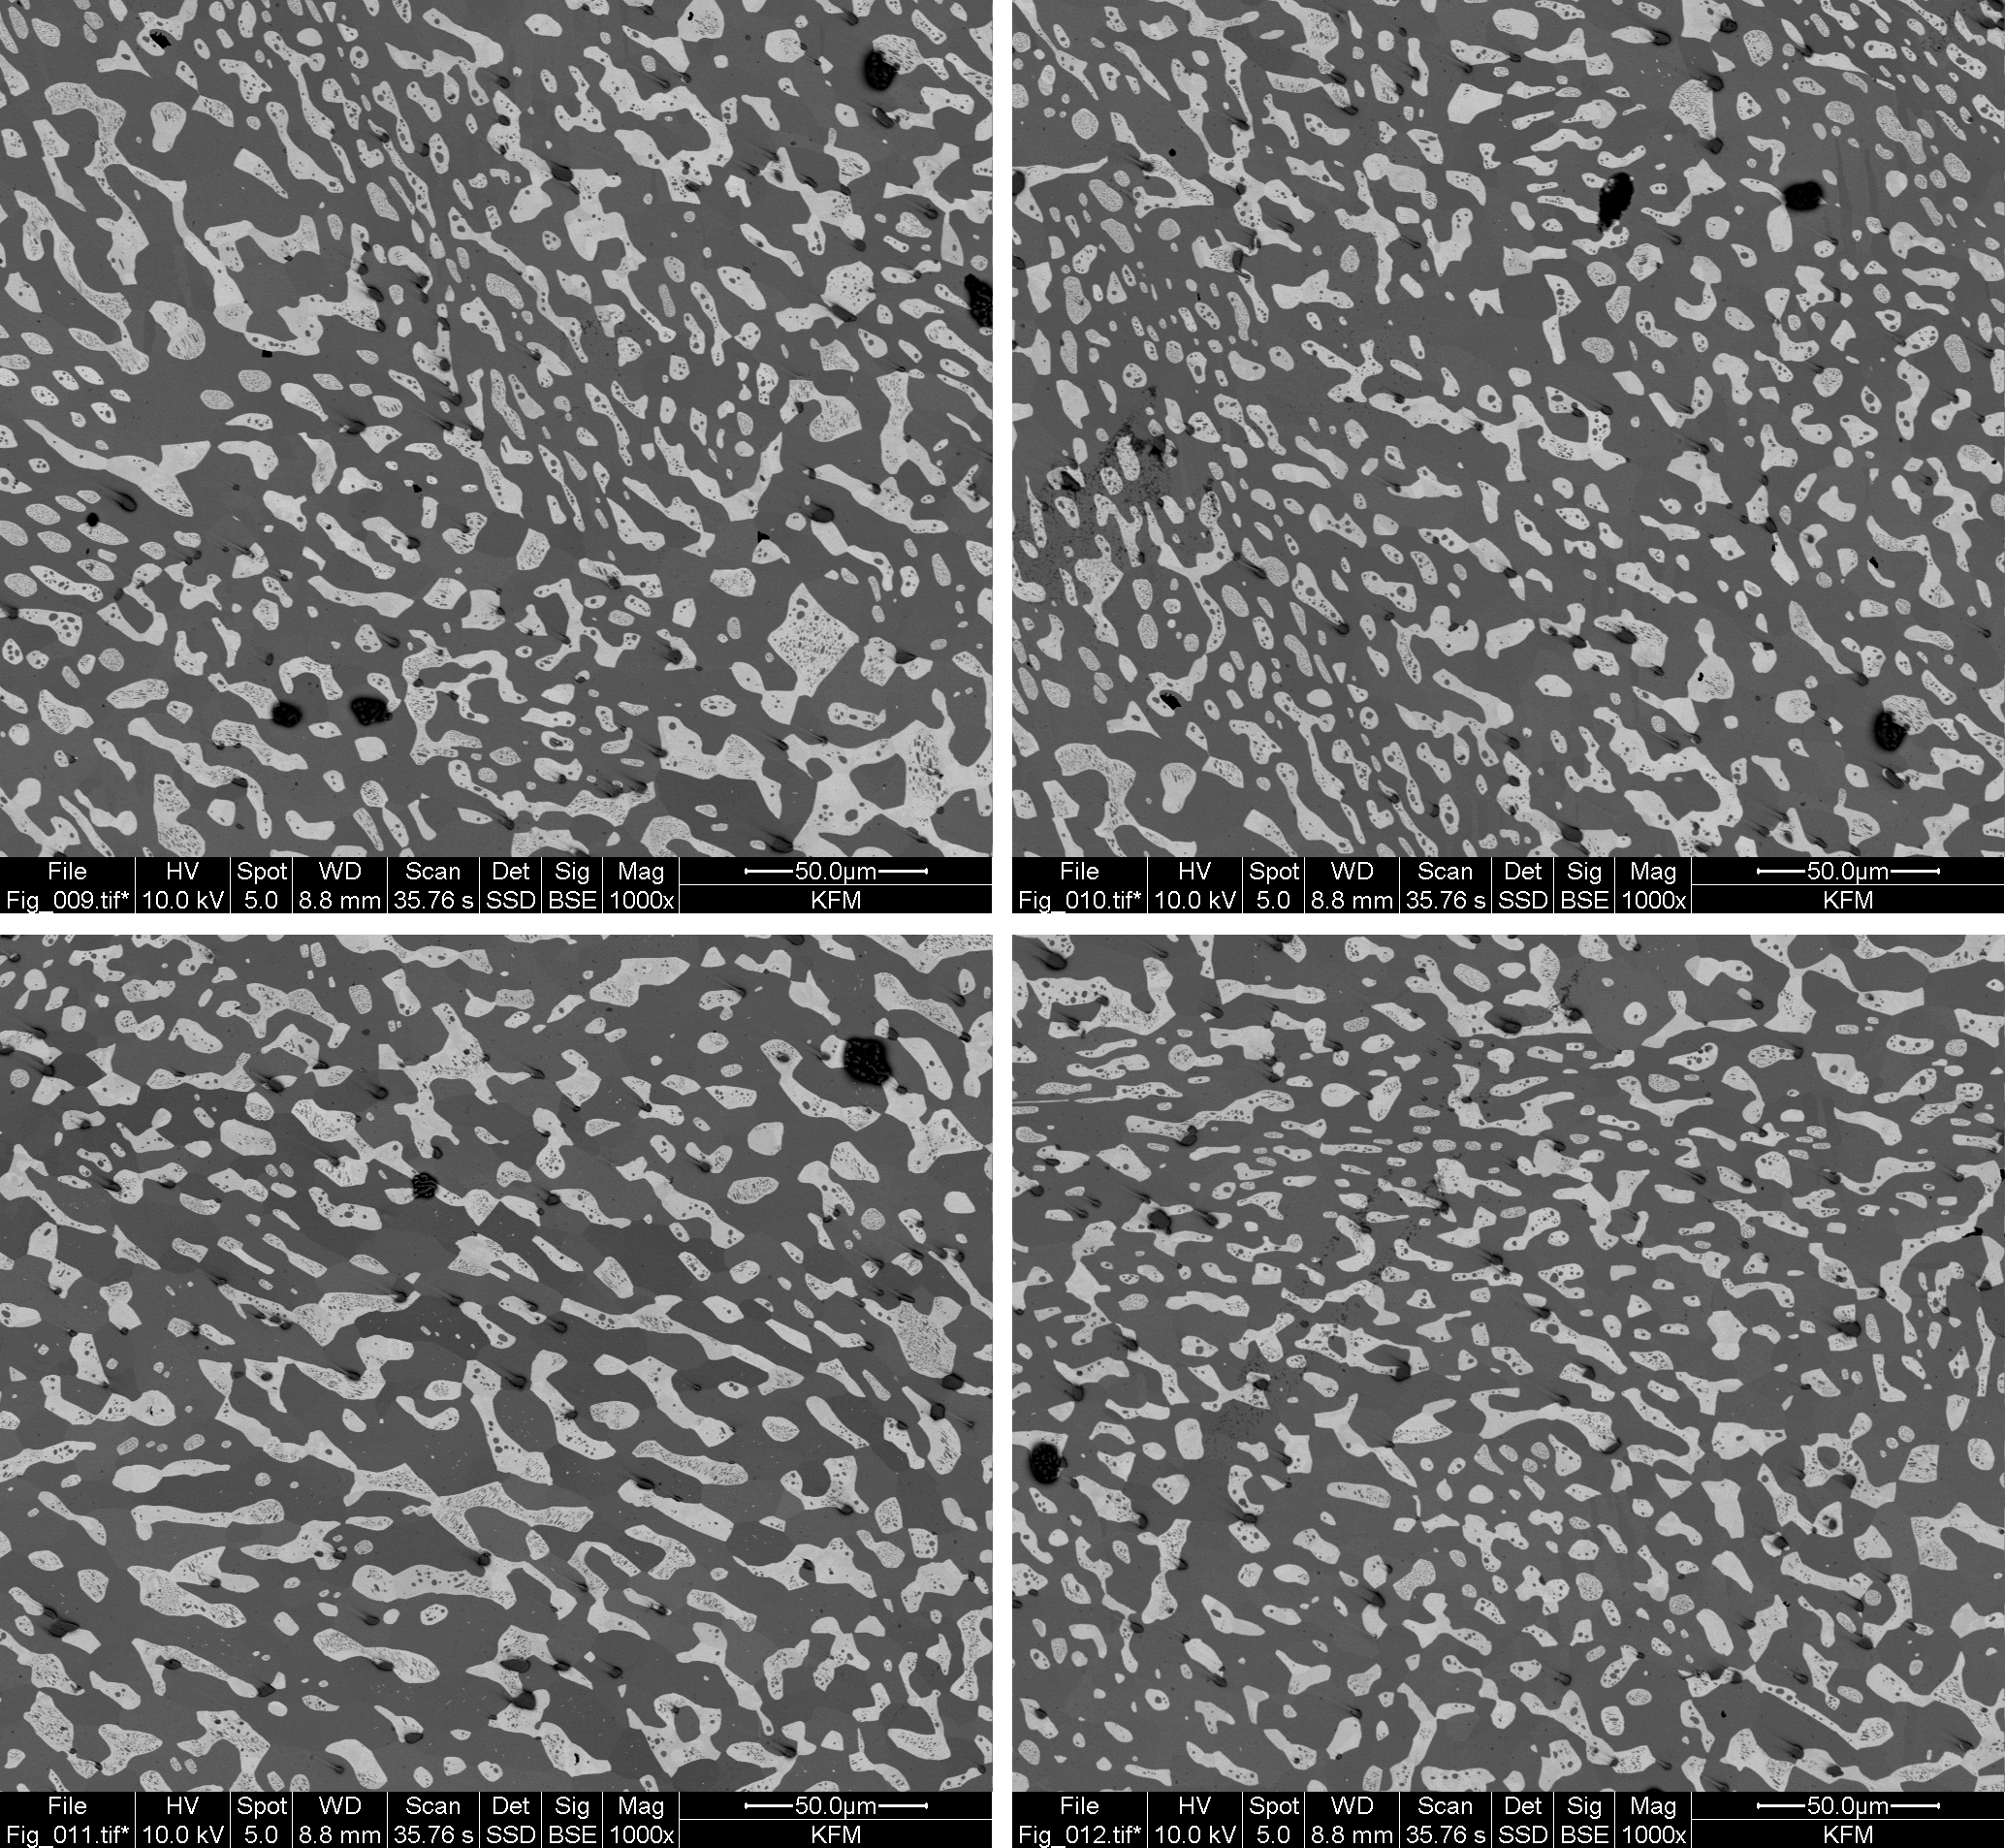
\includegraphics[]{u3}
      \caption{Závislost $U_c(I_{mag})$ pro čtyři poloměry zakřivení dráhy elektronů}
      \label{fig:u3}
    \end{figure}

    Parametry $k$ fitů jsou 
    $$ k_{r=\SI{20}{mm}} = \SI{15.83 \pm 0.08}{\volt\per\ampere\squared}, $$
    $$ k_{r=\SI{30}{mm}} = \SI{37.63 \pm 0.19}{\volt\per\ampere\squared}, $$
    $$ k_{r=\SI{40}{mm}} = \SI{68.0 \pm 0.6}{\volt\per\ampere\squared}, $$
    $$ k_{r=\SI{50}{mm}} = \SI{108.4 \pm 1.1}{\volt\per\ampere\squared}. $$

    Podle rovnice \eqref{eq:k} jsme získali hodnoty měrného náboje 
    $$ \left(\frac{e}{m_e}\right)_{r=\SI{20}{mm}} = \SI{1.65 \pm 0.17}{\coulomb\per\kilogram}, $$
    $$ \left(\frac{e}{m_e}\right)_{r=\SI{30}{mm}} = \SI{1.74 \pm 0.12}{\coulomb\per\kilogram}, $$
    $$ \left(\frac{e}{m_e}\right)_{r=\SI{40}{mm}} = \SI{1.77 \pm 0.09}{\coulomb\per\kilogram}, $$
    $$ \left(\frac{e}{m_e}\right)_{r=\SI{50}{mm}} = \SI{1.81 \pm 0.07}{\coulomb\per\kilogram}. $$
    Chybu hodnot poloměrů jsme určili na $\SI{1}{mm}$.
  
  \section*{Diskuse}

    Všechny získané hodnoty měrného náboje v rámci uvedené chyby odpovídají tabulkové hodnotě. Je zřejmé, že hodnoty určené pomocí dráhy elektronů s větším poloměrem křivosti jsou přesnější, především díky menší relativní chybě tohoto poloměru. Je dále zřejmé, že měření trpí jistou systematickou chybou, protože hodnoty s vyšším poloměrem již hodnotu měrného náboje nadhodnocují. Tato systematická chyba se též projevila v grafu \ref{fig:u3}, kde jsme ve fitovací funkci museli přidat aditivní konstantu, protože naměřené závislosti neprocházely nulou.

  \section*{Závěr}

    Hodnoty měrného náboje určené v tomto praktiku jsou 

    $$ \left(\frac{e}{m_e}\right)_{r=\SI{20}{mm}} = \SI{1.65 \pm 0.17}{\coulomb\per\kilogram}, $$
    $$ \left(\frac{e}{m_e}\right)_{r=\SI{30}{mm}} = \SI{1.74 \pm 0.12}{\coulomb\per\kilogram}, $$
    $$ \left(\frac{e}{m_e}\right)_{r=\SI{40}{mm}} = \SI{1.77 \pm 0.09}{\coulomb\per\kilogram}, $$
    $$ \left(\frac{e}{m_e}\right)_{r=\SI{50}{mm}} = \SI{1.81 \pm 0.07}{\coulomb\per\kilogram}. $$

  \begin{thebibliography}{}
 
    \bibitem{pokyny}
    Pokyny k měření ``Určení měrného náboje elektronu z trajektorie ve zkřížených polích'', dostupné z\\ \url{https://physics.mff.cuni.cz/vyuka/zfp/_media/zadani/texty/txt_423.pdf}, 23.\,10.\,2018
   
  \end{thebibliography}

\end{document} 